% Latex template: mahmoud.s.fahmy@students.kasralainy.edu.eg
% For more details: https://www.sharelatex.com/learn/Beamer

\documentclass[aspectratio=1610]{beamer}					% Document class

\setbeamertemplate{footline}[text line]{%
  \parbox{\linewidth}{\vspace*{-8pt}Perspectives on GBP5 transcriptional bursting, chromatin structure, and transcriptional condensates \hfill\insertshortauthor\hfill\insertpagenumber}}
\setbeamertemplate{navigation symbols}{}

\usepackage[english]{babel}				% Set language
\usepackage[utf8x]{inputenc}			% Set encoding

\mode<presentation>						% Set options
{
  \usetheme{default}					% Set theme
  \usecolortheme{default} 				% Set colors
  \usefonttheme{default}  				% Set font theme
  \setbeamertemplate{caption}[numbered]	% Set caption to be numbered
}

% Uncomment this to have the outline at the beginning of each section highlighted.
%\AtBeginSection[]
%{
%  \begin{frame}{Outline}
%    \tableofcontents[currentsection]
%  \end{frame}
\usepackage{graphicx}					% For including figures
\usepackage{booktabs}					% For table rules
\usepackage{hyperref}	
\usepackage{tikz-network}				% For cross-referencing
\usepackage[absolute,overlay]{textpos}
\usepackage{bm}
\usepackage[font=small,labelfont=bf]{caption}				% For cross-referencing

\title{Perspectives on GBP5 transcriptional bursting, chromatin structure, and transcriptional condensates}	% Presentation title
\author{Clayton W. Seitz}								% Presentation author
\date{\today}									% Today's date	

\begin{document}

% Title page
% This page includes the informations defined earlier including title, author/s, affiliation/s and the date
\begin{frame}
  \titlepage
\end{frame}


% The following is the most frequently used slide types in beamer
% The slide structure is as follows:
%
%\begin{frame}{<slide-title>}
%	<content>
%\end{frame}

\begin{frame}{Current events}
\begin{itemize}
\item GBP5 transcriptional kinetics are changed after Interferon-$\gamma$ priming (Siwek 2020; Molecular Cell) - we have now observed this also
\item HiC data shows Interferon-$\gamma$ causes chromatin reorganization at GBP5 locus (Platinitis 2022; Science)
\item Phase separated condensates are responsible for decrease in the degree of disorder of chromatin at macrophage GBP5 locus during bacterial infection (Lin 2022; Nature Comm)
\end{itemize}
\vspace{0.2in}
Are persistent transcriptional condensates responsible for the change in GBP5 transcriptional kinetics?

\end{frame}

\begin{frame}{A modern view of transcriptional control}
\begin{figure}
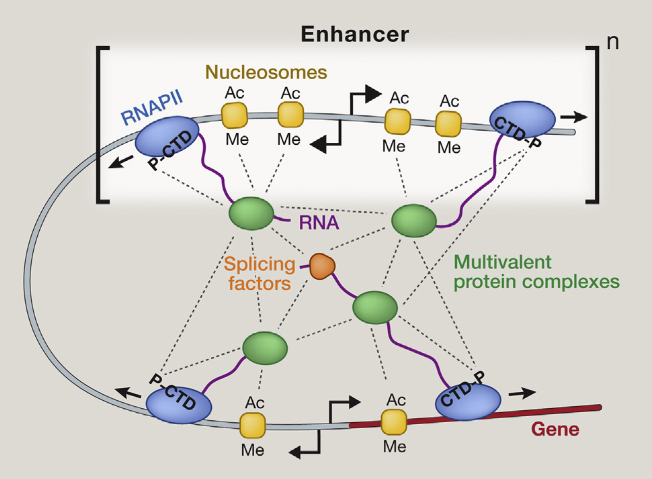
\includegraphics[width=10cm]{figure-5-6.png}
\end{figure}
\end{frame}

\begin{frame}{Super-enhancers host large molecular complexes that facilitate transcription}
\begin{figure}
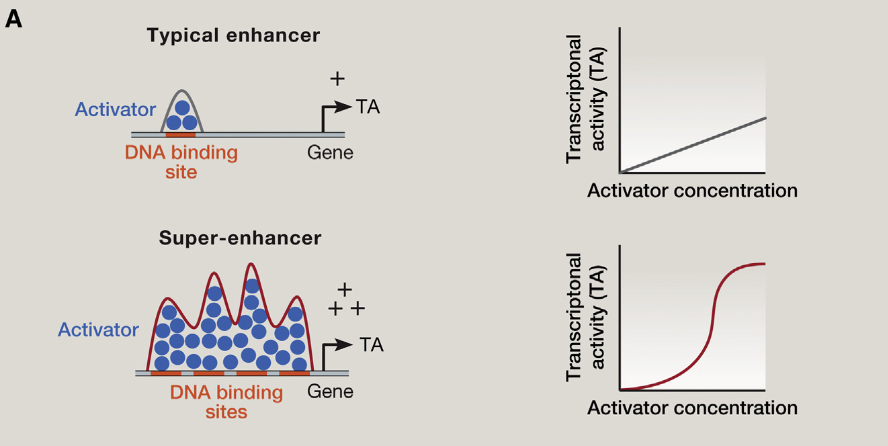
\includegraphics[width=14cm]{figure-5-1.png}
\end{figure}
\end{frame}

\begin{frame}{Super-enhancers host large molecular complexes that facilitate transcription}
\begin{figure}
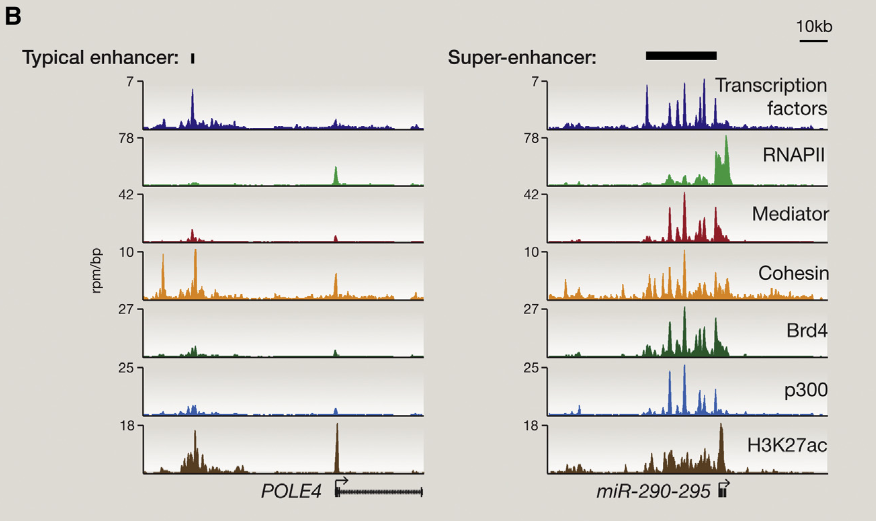
\includegraphics[width=12cm]{figure-5-2.png}
\end{figure}
\end{frame}

\begin{frame}{Structural modeling of phase-separated aggregates}
\begin{figure}
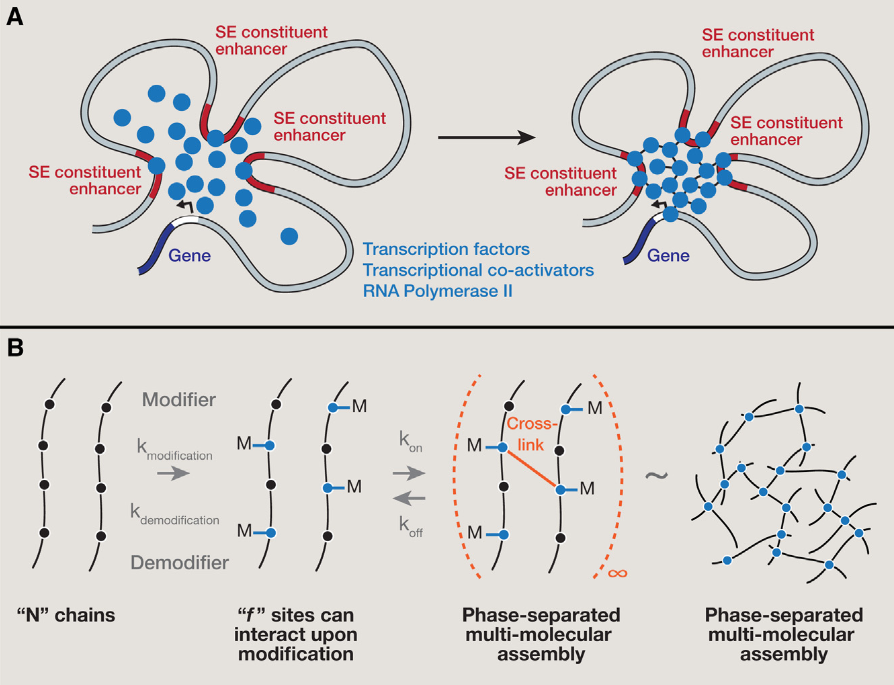
\includegraphics[width=10cm]{figure-5-3.png}
\end{figure}
\end{frame}


\begin{frame}{The role of valency in phase-separated aggregates}
\begin{figure}
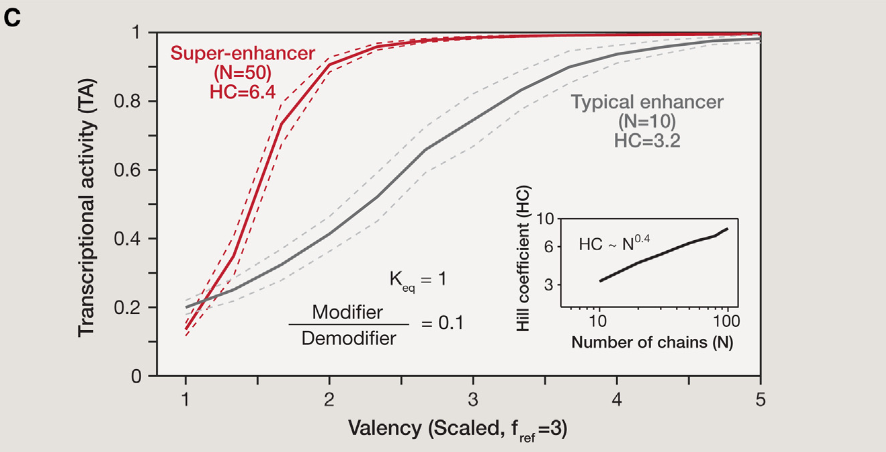
\includegraphics[width=14cm]{figure-5-4.png}
\end{figure}
\end{frame}

\begin{frame}{Phase separation inhibitor JQ1 reduces transcription}
\begin{figure}
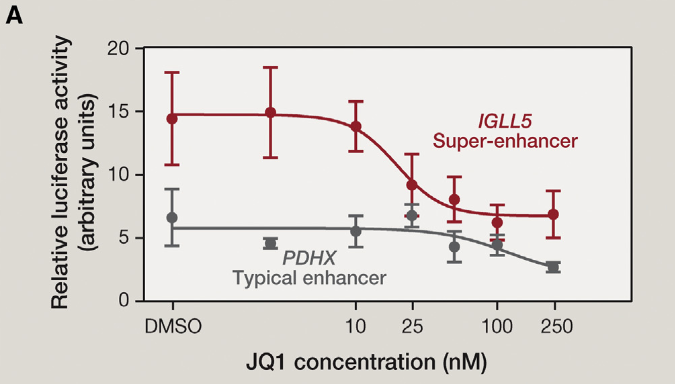
\includegraphics[width=12cm]{figure-5-5.png}
\end{figure}
\end{frame}

\begin{frame}{Super-enhancers reduce transcriptional variability in \emph{Drosophila} embryos}
\begin{figure}
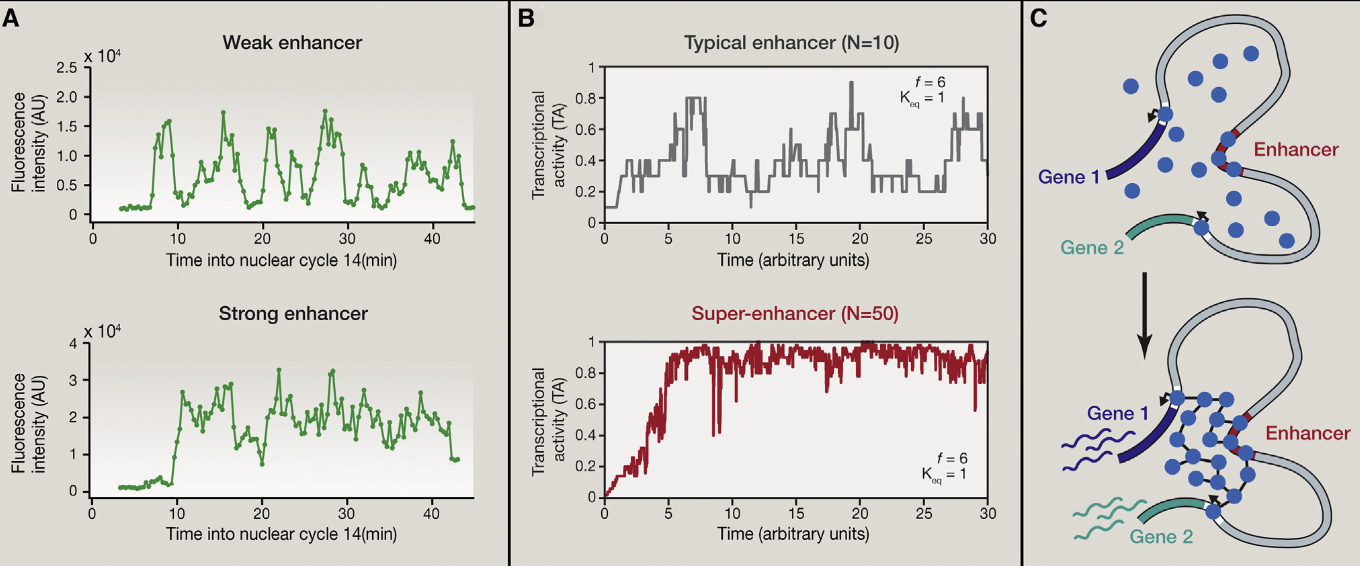
\includegraphics[width=14cm]{figure-5-7.png}
\end{figure}
\end{frame}


\begin{frame}{}
\begin{figure}
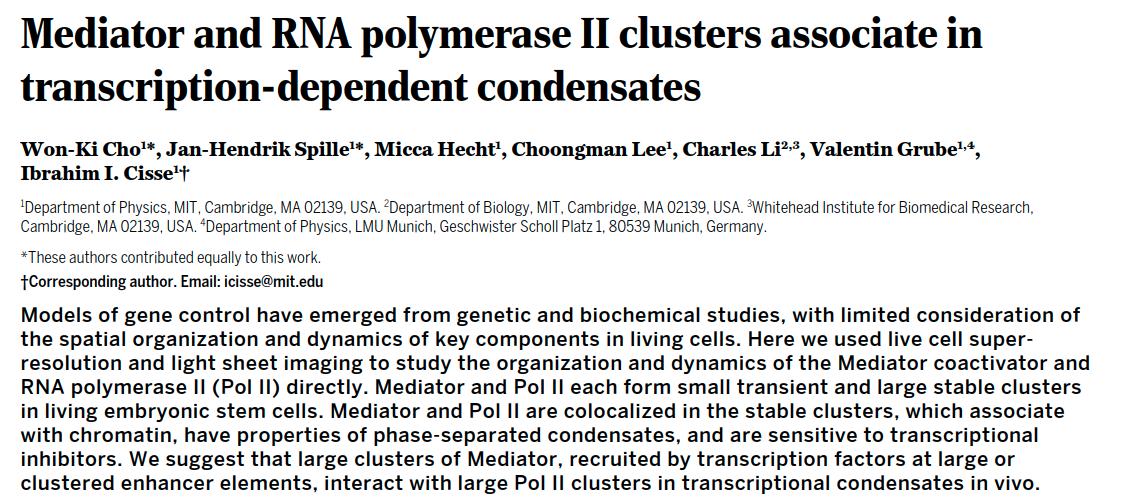
\includegraphics[width=14cm]{abstract-1.png}
\end{figure}
\end{frame}


\begin{frame}{Mediator and Pol II form transient and stable clusters}
\begin{figure}
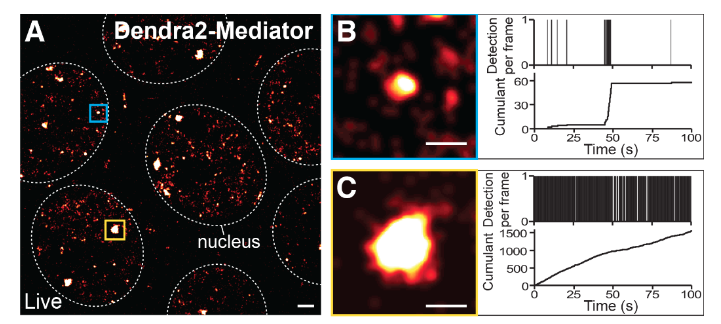
\includegraphics[width=14cm]{figure-1-1.png}
\end{figure}
\end{frame}


\begin{frame}{Mediator and Pol II form transient and stable clusters}
\begin{figure}
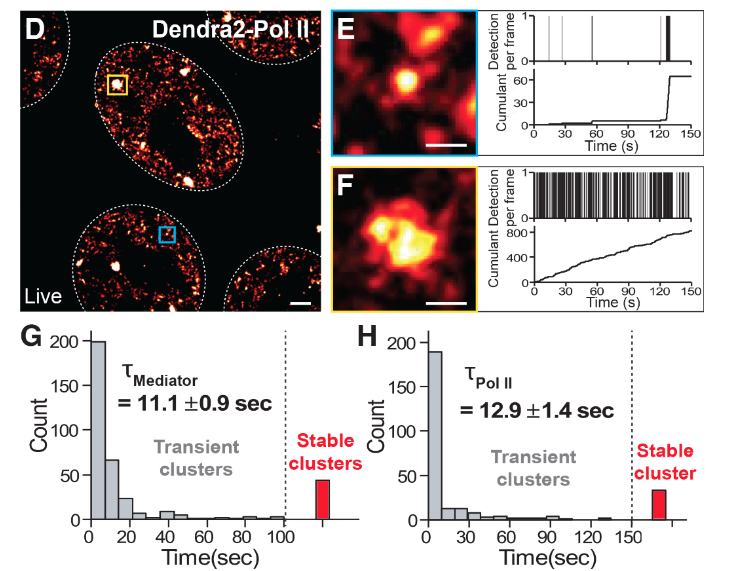
\includegraphics[width=10cm]{figure-1-2.png}
\end{figure}
\end{frame}


\begin{frame}{Mediator  and  Pol  II  clusters  colocalize  in  a  transcription  dependent  manner}
\begin{figure}
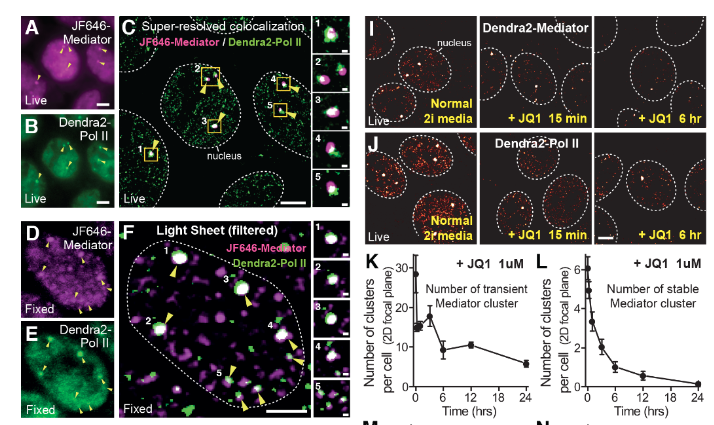
\includegraphics[width=14cm]{figure-2-1.png}
\end{figure}
\end{frame}


\begin{frame}{Mediator   clusters   dynamically   kiss   actively  transcribing SE-controlled  genes}
\begin{figure}
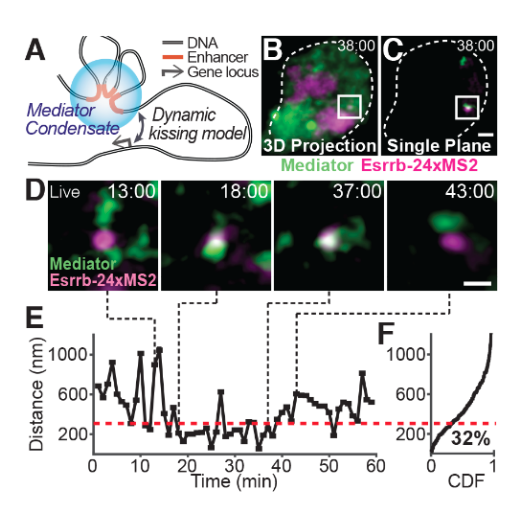
\includegraphics[width=8cm]{figure-3-1.png}
\end{figure}
\end{frame}



\end{document}